%%
%% This is file `minimal_imlex.en.tex',
%% generated with the docstrip utility.
%%
%% The original source files were:
%%
%% uefcsthesis.dtx  (with options: `ex,en,modern,imlex')
%% 
%% This is a generated file.
%% 
%% Copyright (C) 2018--2022 by Pauli Miettinen <pauli.miettinen@uef.fi>
%% 
%% This file may be distributed and/or modified under the conditions of
%% the LaTeX Project Public License, either version 1.3c of this license
%% or (at your option) any later version.  The latest version of this
%% license is in:
%% 
%% http://www.latex-project.org/lppl.txt
%% 
%% and version 1.3c or later is part of all distributions of LaTeX
%% version 2006/05/20 or later.
%% 
%% 
%% This is a minimal example of using the uefcsthesis class.
%% This generates an English MSc thesis with one-sided layout.
%% To compile, use either lualatex or xelatex, for example,
%% $ lualatex minimal_modern.en.tex
%% $ biber minimal_modern.en
%% $ lualatex minimal_modern.en.tex
%% or use latexmk:
%% $ latexmk -lualatex minimal_modern.en.tex
%%
%% When returning the final thesis to library, you must also return the source code
%% used to create the final version. This is easiest if you flatten your document into
%% a single file (+ image files). To do that, use can use latexpand (see
%% https://www.ctan.org/pkg/latexpand), which is also part of TeX Live and
%% MiKTeX packages. An example use of latexpand would be
%% $ lualatex minimal_modern.en.tex
%% $ biber minimal_modern.en
%% $ latexpand --empty-comments --biber minimal_modern.en.bbl \
%% > minimal_modern.en.tex > flat_thesis.tex
%% $ lualatex flat_thesis
%% $ lualatex flat_thesis
%% which produces files called flat_thesis.tex and flat_thesis.pdf that can be
%% returned to the library.
%%

\documentclass[mscthesis,english,oneside,biblatex,imlex]{template/uefcsthesis}
%% Correct the below with the name of your bibliography file
\addbibresource{bibliography.bib}
\usepackage{txfonts}

% Fabiano: these are packages added by me:
\usepackage[dvipsnames]{xcolor}  % enables textcolor
\usepackage[acronym, toc]{glossaries}  % enables glossaries
\usepackage{lastpage}
\usepackage{fancyhdr}


%% Replace all capital text with your own information.
\title{Text-based Person re-Identification for human tracking} % Title of the thesis
\author{Yuya}{Takagi} % Your name
\date{\thismonth} % The month and year of handing in your thesis, or \thismonth of automatic
\city{Joensuu} % Either Kuopio or Joensuu
\firstsupervisor{Jun Miura} % Name of the first supervisor
\keywords{ Text-based person Re-identification\sep Textt-based person retrieval} % Keywords must be separated with \sep

%% To get the ACM CCS classification, you can visit
%% https://dl.acm.org/ccs/ccs.cfm
%% There you can find a tool to generate LaTeX code for the classification
%% Copy it here. You don't need to copy the XML at the begin, though.
%% For example,
%% \ccsdesc[500]{Some Class}

%% You can change department, faculty, and university names using the
%% following commands (for now commented out)
%% \setstring{universityname}{Toyohashi University of Technology}
%% \setstring{facultyname}{Faculty of Robotics}
%% \setstring{departmentname}{Department of Computer Science}
%% If you need to use different languages, use \setstring[lang]{<stringname>}{<text>}.
%% You can use \setstring to add translations to all strings in title and abstract
%% pages, see uefcsthesis.pdf, section ``Pre-Defined Strings and a Macro to Change
%% Them'' for further information.


% Fabiano: glossaries stuff, like terms and acronyms.
\makenoidxglossaries
\newglossaryentry{maths}
{
    name=mathematics,
    description={Mathematics is what mathematicians do}
}

\begin{document}
\maketitle

% \begin{abstract}
% Person re-identification is used to 
    
% \end{abstract}

\frontmatter
\tableofcontents
\mainmatter



% Each chapter is separated into a different .tex file. Include them here.
\chapter{Introduction}
Person re-identification is a crucial topic with applications in service robotics and security. The goal is to extract features from an input source and compare them against a large dataset to identify the corresponding individual. Traditional methods predominantly rely on image-based inputs, but these methods face significant challenges due to intra-class variations caused by different viewing angles, environmental changes, and color variations.

To address these issues, with advances in learned models of natural language processing, vision language models are used. There are few methods to train the vision-language models. 
Contrastive training is a common strategy that utilizes pairs of positive and negative examples. In this method, the VLM is trained to produce similar representations for positive pairs and different representations for negative pairs. Another strategy is masking, where the VLM learns to reconstruct missing patches from an unmasked text caption. Similarly, masking words in a caption allows the VLM to reconstruct those words using an unmasked image.

While many approaches use intermediate representations or partial reconstructions, generative VLMs are designed to generate entire images or lengthy captions. Due to their complexity, these models are often the most expensive to train. VLMs with pretrained backbones frequently employ open-source LLMs like Llama to establish a mapping between a pre-trained image encoder and the LLM. It's important to note that these paradigms are not mutually exclusive; many approaches combine contrastive, masking, and generative criteria.

Especially for person retrieval tasks, VLM are trained with combination of contrastive learning and masking. It utilized BERT as the text encoder and Vision Transformer as the image encoder. Typically, the text encoder employs a fixed masking ratio for the masked language modeling (MLM) tasks. This thesis investigates the impact of varying the masking ratio during the training of the visual language model, aiming to understand how these changes affect the model's performance.

\section{Motivation}
The increasing potential for robots to collaborate with humans in various work environments necessitates the development of intuitive communication methods. The most natural way for humans to interact is through text or spoken information. By enabling robots to understand and respond to these forms of communication, we can significantly enhance human-robot collaboration.

Such advancements could address critical issues like manpower shortages by allowing robots to seamlessly integrate into human workforces. To achieve this level of interaction, it is essential to effectively connect and interpret information from both text and images. This requires developing a cross-modal model that can map and recognize features across these different types of data. By focusing on creating such a model, we aim to bridge the gap between text and image information, facilitating more intuitive and efficient human-robot collaboration.

\section{Objectives}
we will tackle through the attention differences between text and image information
previous methods worked on getting better multi-modal representation 
many approaches have been produced, but when we look into mlm models, they do not change the masking ratio. there are studies that had a question about this, but it did not go beyond to person retrieval models. we would like to look into this and see if the accuracy will change.

\section{Document structure}

This paper consists of chapters. Chapter 1 presents the purpose and background of this research and the structure of this paper. Chapter 2 describes the previous findings and theories related to this research. Chapter 3 includes the experiments towards the affect of masking ratio for masked language modeling. Chapter 4 will have a discussion from chapter 3. Chapter 5 presents the conclusions, limitaitons, and future perspectives of this study.

\chapter{Theoretical Background}

\section{LiDAR}

\section{SLAM}

\chapter{Literature Review}


% ------------------------------------------------------------ %


\section{Research Methodology}
\textcolor{red}{WIP}\\
In the methodology section, the we first delves into the existing literature, drawing from a paper accessible through the platform "Paper with Code." This platform typically provides research papers along with their associated code implementations. The chosen paper appears to be selected based on its prominence, likely measured by its reported accuracy or success in the field.
Following the identification of the primary paper, the researcher conducts a thorough review of its content, focusing particularly on aspects related to methodology. This involves understanding the proposed techniques, algorithms, and approaches presented in the paper to achieve high accuracy in the context of text-based person searches. The aim is to comprehend the nuances of the existing methodology and identify the key factors contributing to its success.
In addition to the primary paper, the researcher examines two other papers that exhibit a significant difference in accuracy. This comparative analysis is valuable for gaining insights into different approaches within the field. The choice of these additional papers may be strategic, aiming to capture diverse perspectives or methodologies, especially if there is a notable contrast in their reported accuracy metrics.
The researcher likely scrutinizes the methodologies of these selected papers, comparing and contrasting them with the primary paper. This comparative analysis helps identify the strengths and weaknesses of different approaches, shedding light on potential areas of improvement or innovation for the current research.
Overall, the methodology involves a comprehensive exploration of relevant literature, with a focus on the primary paper selected from "Paper with Code." The intent is to understand the methodologies employed in achieving high accuracies and to leverage insights from other papers with varying performance metrics. 

However, if only paperwithcode is used, the information obtained is limited and biased. To eliminate this bias, we decided to use scopus to search a wider range of papers by keyword search.

\subsection*{Identification}

The following research question was defined:

\bigskip
\textit{``How can we discern and identify the details of a person in text-based person search?''}
\bigskip


From this research question, four main keywords that sufficiently explain the topic were used: person retrieval and vision language pre-training.
Furthermore, synonyms and related terms were associated to these keywords to form keyword groups as follows:

\begin{itemize}
    \item person retrieval:
    \begin{itemize}
        \item person;
        \item person detection;
        \item person search.
    \end{itemize}
    \item vision language pre-training:
    \begin{itemize}
        \item VLP;
        \item text based;
        \item text.
    \end{itemize}
\end{itemize}


From the keywords, we had a keyword search on scopus from the search strings as follows:

\begin{itemize}
    \item ( "person retrieval" OR "person" OR "person detection" OR "person search" ) AND ( "vision language pre-training" OR "VLP" OR "text based" OR "text" ).
\end{itemize}

The Scopus search yielded a total of $20170$ documents. Within this result, we set the subject area to Computer Science, document type to article and conference paper, language to only english, and set the open access to all open access. With this filters, $862$ articles were found. 

\subsection*{Screening}

Various factors were taken into account for the exclusion of documents:
\begin{enumerate}
    \item problem and goal were too different (e.g., building new hardware, analysis of leaf reflectance);
    \item not sufficiently related to this work (e.g., focused on hyperspectral );
    \item duplicates that were not automatically detected and excluded.
\end{enumerate}



% ------------------------------------------------------------ %

\section{Transformer}
The Transformer was initially introduced for machine translation within the realm of natural language processing (NLP)\cite{vaswani2023attention}. Previous NLP models utilizes convolutional neural networks(CNN) or recurrent neural networks(RNN) for encoder and decoder. However, training this model is time consuming and required tremendous amount of labeled datasets. The transformer solves those problems by implementing an attention unit. 

\section{Vision-language pre-training}
Vision language pre-training has drawn increasing attention after Transformer came up. Transformer is meant for NLP tasks, but the researcher found out that this model is capable of many tasks including information retrieval from the image, classification, etc. Since then, many follow-up works are proposed, such as BERT, CLIP, RoBERTa, GPT series. 
we know that bigger the transformer layer, the better accuracy. some methods like gpt4 has billions of parameters 
there are research that seeks into less parameters, enabling small model with efficient accuracies.

vision language like 
vibert
albef 
CLIP


\section{Person Understanding Task}
in this section we will talk about different method we can use for person understanding task. 
\subsection{Text-based re-identification}
\textcolor{red}{WIP}\\
This section presents papers that study text-based person retrieval. A common issue addressed in each paper is the deficiency of the feature from text and image encoders. It has been confirmed that when the features of each modal are integrated, information is distorted or missing, which affects the accuracy of detection. Therefore, how to resolve this deficiency is key in this section.

\subsubsection{RaSa: Relation and Sensitivity Aware e Representation Learning for Text-based Person Search}
\textcolor{red}{WIP}\\
This paper introduces a method called Relation and Sensitivity Aware representation learning (RaSa) that includes two novel tasks: Relation-Aware learning (RA) and Sensitivity-Aware learning (SA). It addresses the shortcomings of existing methods in text-based person search, where clustering representations of positive pairs without distinction leads to overfitting, particularly with weak positive pairs. RA mitigates overfitting by introducing a positive relation detection task to distinguish between strong and weak positive pairs. Additionally, the author emphasizes the common practice of learning invariant representation under data augmentation for robustness but goes further by encouraging the representation to perceive sensitive transformations through SA, promoting enhanced robustness by detecting replaced words in textual descriptions.

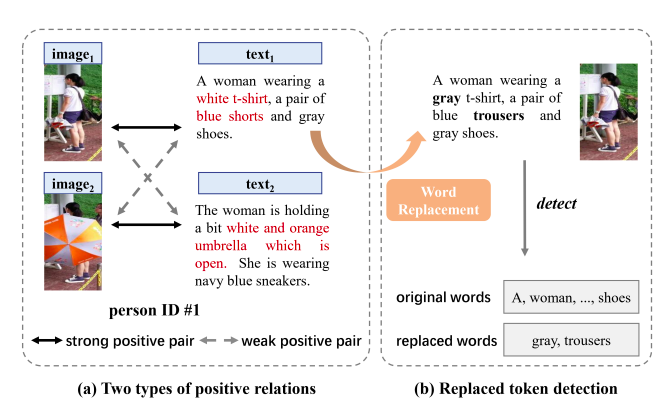
\includegraphics[width=10cm]{img/rasa.png}


\subsubsection{Cross-Modal Implicit Relation Reasoning and Aligning for Text-to-Image Person Retrieval}
The paper introduces a novel approach, called IRRA (Implicit Relation Reasoning and Aligning), for text-to-image person retrieval. This task i`nvolves identifying a person based on a given textual description. The main challenge is to establish an effective mapping between visual and textual modalities in a shared latent space. Unlike previous methods that use separately pre-trained unimodal models, IRRA addresses this challenge by introducing a cross-modal Implicit Relation Reasoning module. This module integrates visual cues into textual tokens through a masked language modeling paradigm, facilitating cross-modal interaction. To globally align visual and textual embeddings, the paper proposes Similarity Distribution Matching, which minimizes the KL divergence between image-text similarity distributions and normalized label matching distributions. 

\subsubsection{Learning Semantic-Aligned Feature Representation for Text-based Person Search}
The paper focuses on text-based person search, aiming to retrieve images of a specific pedestrian based on a textual description. The primary challenge in this task is to bridge the inter-modality gap and align features across textual and visual modalities. The proposed solution is a semantic-aligned embedding method that automatically learns feature alignment between visual and textual representations. The method utilizes two Transformer-based backbones to encode robust feature representations for images and texts. Additionally, a semantic-aligned feature aggregation network is introduced, incorporating a multi-head attention module constrained by a cross-modality part alignment loss and a diversity loss. 


\subsection{Image-based re-identification}
with the image based methods, we have the old fashion way of cnn 


\subsection{person attribute recognition}
person attribute recognintion has seeked to have supervision 
... made a mask on the person to set the person 
... tried to slice the image so that we can extract specific parts from the person
... tried to create a filter 

% ------------------------------------------------------------ %

\chapter{Proposed Methods}

% do i need this
% In this chapter, we introduce the proposed methods and experimental methodology. This research aims to address the question, "What would happen if we change the masking strategies?" While numerous strategies have been proposed to enhance the representation of text and images, there has been limited experimentation on altering the masking ratio in masked language modeling (MLM). This study primarily focuses on two main aspects:

% \begin{itemize}
%   \item The referenced model employs masked language modeling to train feature extraction, maintaining a constant masking ratio throughout the training process. This research proposes varying the masking ratio and introducing a time-variant component during training.
%   \item The referenced model includes a function known as momentum-based replace token detection, which also operates with a specific masking ratio. This study examines whether adjusting the masking ratio for this task, similar to the approach taken with MLM, improves prediction performance when both parameters are modified.
% \end{itemize}
%%%

% \color{WIP}
% The purpose of this experiment is to examine the hypothesis that time variant masking ratio affect the prediction on text based person retrieval.
% This is carried out by investigating the relation and sensitivity aware representation learning \cite{Bai2023RaSaRA} that investigated the better representation learning for image and text inputs by detecting the replaced tokens from the converted text and corresponding image inputs. The results showed significant improvements in prediction performance. To investigate further towards the masking ratio, \cite{wettig-etal-2023-mask} investigated that larger models should adopt a higher masking rate rather than masking 15\% of tokens conventionally. Another method from Dongjie Yang, et al, \cite{yang2023learningbettermaskingbetter} proposed time-variant masking ratio decay strategy and POS-tagging weighed masking. In results, the time variant masking decay method outperformed the time invariant masking ratio for F1 score on SQuAD performance during pre-training on BERT-large model. 

The purpose of this experiment is to examine the hypothesis that a time-variant masking ratio would affects the prediction accuracy in text-based person retrieval tasks. We approach this by exploring the relationship between the sensitivity-aware representation learning, as investigated by Bai et al. (\cite{Bai2023RaSaRA}) in their work "RaSa," which focuses on improving representation learning for image and text inputs by detecting replaced tokens from the combined text and image inputs. Their results demonstrated significant improvements in prediction performance. They used masked language modeling to combine the image and text feature to match the information, but the masking ratio were fixed to 15\% during the whole process.

To delve deeper into the impact of masking ratios, (\cite{wettig-etal-2023-mask}) suggested that larger models benefit from adopting a higher masking rate rather than the  conventional 15\% of tokens. Additionally, (\cite{yang2023learningbettermaskingbetter}) proposed a time-variant masking ratio decay strategy along with POS-tagging weighted masking. Their findings indicated that the time-variant masking decay method significantly outperformed the time-invariant masking ratio in terms of F1 score on the SQuAD dataset during the pre-training of the BERT-large model.

Our experiment aims to build on these insights by evaluating the effects of different masking strategies on the performance of vision-language models, specifically in the context of text-based person retrieval. By systematically varying the masking ratio and employing time-variant masking techniques, we seek to determine the optimal approach for enhancing the alignment and interpretation of textual and visual data.

% this part might not required
In this experiment, we investigate the effect of the performance towards the time variant masking ratio on replaced token detection task. To evaluate the performance, we will compute the feature similarity score for all image-text pairs. Then we take top-$k$ candidates and calculate their ITM score $s_{itm}$ for ranking. 

\section{Dataset}

\begin{figure}[htbp]
  \begin{center}
      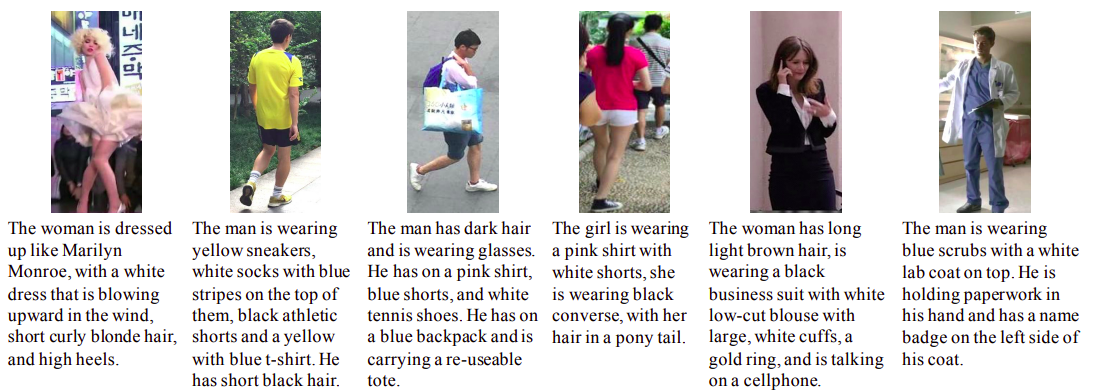
\includegraphics[width=\linewidth]{img/cuhk_pedes.png}
      \caption{Example sentence with corresponding image}
      \label{fig:cuhk_pedes}
  \end{center}
\end{figure}


Dataset we are using is CUHK-PEDES \cite{li2017personsearchnaturallanguage}. This is a large-scale dataset created to facilitate person search using natural language descriptions. It addresses the need for a dataset where persons are described in detail using natural language, enabling practical applications such as video surveillance. Key features of the dataset are shown as follows:
\begin{itemize}
  \item Large-scale: Dataset contains 40,206 images over 13,003 persons 
  \item Annotations: Each images is described with two sentences by independent annotators, in total of 80,412 sentence descriptions
  \item Source diversity: Images are sourced from a variety of existing person re-identification datasets, including CUHK03\cite{li2014deepreid}, Market-1501\cite{7410490}, SSM\cite{ssm}, VIPeR\cite{viper}, and CUHK01\cite{li2012human}.
\end{itemize}

The datasets contains image and corresponding natural language description as shown in Fig\ref{fig:cuhk_pedes}. Image source for CUHK-PEDES are from CUHK03, Market-1501, SSM, VIPER, and CUHK01. The annotations for each image are done by Amazon Mechanical Turk(AMT), which is a crowd workers that are employed to describe each image with two sentence. Each sentence include rich descriptions about person appearance, action poses, and interactions.

\section{Methods}
In this section, we introduce the experimental methods designed to evaluate the performance of vision-language models (VLMs). Recent state-of-the-art VLMs, such as the one described by Bai et al. (2023) in their work "RaSa," utilize an attention mechanism to extract and align features from both images and text using cross-modality encoders. Achieving optimal results necessitates not only robust feature extraction but also the development of sophisticated textual representations to enhance the interpretation of visual data. Therefore, our objective is to train the visual-language model (Bai et al., 2023) by employing diverse strategies for textual information representation. Specifically, we will investigate two distinct methods to determine their impact on model performance.

% explain about the parameters based on the model image and loss function

\subsection{Masking ratio for masked language modeling} 
A Masked Language Model (MLM) is a type of neural network model used primarily for natural language processing tasks, including (\cite{devlin2018bert}, \cite{Bai2023RaSaRA}). MLMs are trained on text data where some of the words in the input sentences are replaced with a special token (often "[MASK]"), and the model's objective is to predict the original words that were masked. This training method helps the model learns to capture the semantics and syntax of the language, making it effective for various NLP tasks such as text classification, sentiment analysis, and machine translation.

During training, a portion of the input tokens are randomly masked, and the model learns to predict these masked tokens based on the surrounding context. For example, in the sentence "The cat sat on the [MASK]," the model should predict "mat" if it has learned the context correctly. For each image and text pair ($I,T^S$), MLM loss will be formulated as:
\[
  L_{mlm} = \mathbb{E}_{p \left( I,T^{msk}\right) }\mathrm{H}\left(y^{mlm}, \phi^{mlm}\left(I,T^{msk}\right)\right)
\]

Given a masked text \( T_{msk} \), where each token in the input text \( T_s \) is randomly masked with a probability \( p_m \), \( y_{mlm} \) represents a one-hot vector indicating the ground truth of the masked token. The function \( \phi_{mlm}(I, T_{msk}) \) denotes the predicted probability for the masked token, based on the context provided by the masked text \( T_{msk} \) and the paired image \( I \).

% explanation about what we do with masking ratio
In natural language pre-training, masked language modeling is utilized to understand the context of an input sentence. This same task is applied to recent vision-language models, where the masked token is predicted using both the image and the remaining text information. Although this method can yield good performance, the typical ratio for masking words in a sentence is fixed at 15\%. In our study, we aim to identify the optimal masking ratio by experimenting with time-invariant masking ratios ranging from 15\% to 40\%. Additionally, we will explore time-variant masking strategies based on previous findings to further enhance model performance.

% - モデルとパラメータの具体的な説明
% - 始めにどの比率が効果的かの検証
% - 次に時間変動での検証

\subsubsection{fixed masking ratio}
We will train the model with constant masking ratio with range of 15\% to 40\% by 5\% steps with the dataset of CUHK-PEDES. Then, from the results, we will take the most highest mAP from the constant masking ratio and use that value with the minimum masking ratio. The minimum ratio will be 2\% since 0\% masking ratio will not train at all. 

For all training tasks, the number of epochs is set to 30, batch size is 13. With this, the model will train under 30 iterations and trains with the dataset which is divided to 13 different datasets. The optimization methods are adamW, learning rate is set to 1.0e-4 at first and create a cosine curve to decrease to 1.0e-5. 

\begin{tabular}{rcccc}
  masking ratio & r1 & r5 & r10 & mAP\\ \hline
  15\% & 76.51 & 90.20 & 94.25 & 69.38 \\
  20\% & 76.64 & 89.90 & 93.70 & 70.27 \\
  25\% & 76.23 & 89.86 & 93.79 & 70.22 \\
  30\% & 76.72 & 89.77 & 93.60 & 70.30 \\
  35\% & 76.61 & 89.77 & 93.47 & 70.26 \\
  40\% & 76.56 & 89.88 & 93.47 & 70.26
\end{tabular}

\subsubsection{time variant masking ratio}
Time variant strategy will have the cosine curve and linear curve to see the result. The time variant will have four different methods, linear increase, linear decrease, cosine increase, and cosine decrease. The equations are shown as follows:
\begin{displaymath}
  M_{linear increase}(t) = P*t/T \
  M_{linear decrease}(t) = P*(1-t/T) \
  M_{cosine increase}(t) = P*(1-cos(\pi*t/T)) + 0.02 \ 
  M_{cosine decrease}(t) = P*(1+cos(\pi*t/T)) + 0.02 
\end{displaymath}

\begin{tabular}{rcccc}
  masking ratio & r1 & r5 & r10 & mAP\\ \hline
  linear increase & 76.62 & 89.88 & 93.62 & 70.36 \\
  linear decrease & 76.70 & 89.85 & 93.58 & 70.21 \\
  cosine increase & 76.54 & 90.04 & 94.02 & 70.15 \\
  cosine decrease & 76.21 & 90.09 & 93.65 & 70.21 \\
\end{tabular}

\section{masking ratio for replaced token detection}
RaSa utilizes this to create a task called sensitivity aware learning.
Sensitivity aware aims to make the model sensitive to specific transformations in the data, particularly textual changes. While many models aim to learn invariant representations that are robust to various data augmentations, RaSa takes it further by encouraging the model to detect and respond to sensitive transformations, such as word replacements in text. This is done using a Momentum-based Replaced Token Detection (M-RTD) task, where the model learns to detect whether a token in the text has been replaced. This sensitivity to changes enhances the robustness and discrimination power of the representations learned by the model.


Predicting more means the model learns from more training signals, so higher prediction rates boost the model performance. From another perspective, each prediction at each masked token leads to a loss gradient, which is averaged to optimize the weights of the model. Averaging across more predictions has a similar effect to increasing the batch size, which is proved to be beneficial for pre-training (Liu et al., 2019). 

\section{Attention visualization}
To be able to see where the model is paying attention to, we would use the attention matrix in cross atttention module.



\section{Algorithm implementation}

for the 
\chapter{Evaluation}

\section{Test suite}

\section{Experiments}

\section{Results}
% If I add all results to the Evaluation chapter, there's no need for a Results chapter.

% This will depend on how I structure the document once I start writing the experiments and results sections. For now, this stays empty.
\chapter{Discussion}
Discussion will be done for all experiment.
\chapter{Conclusions}
In this study, we explored the impact of various masking strategies on the performance and attention mechanisms of \acrfull{vlm} in the context of text-based person retrieval tasks using the CUHK-PEDES dataset. Our experiments revealed that while different masking ratios can influence specific performance metrics, such as \acrfull{map}, the overall effect on the model's accuracy and robustness remains limited.

The analysis of attention patterns showed that at lower masking ratios, the model tends to focus on finer details within the image, whereas higher masking ratios lead to broader attention across larger image regions. However, a key observation was that the attention to image regions indicated by corresponding words in the text remains stable across different masking strategies. This consistency underscores the model's ability to maintain robust and meaningful connections between textual descriptions and visual features, even when varying the level of masked data during training.

These findings contribute to a deeper understanding of how \acrshort{vlm} process and align multi-modal data, highlighting the importance of attention mechanisms in maintaining consistency and robustness in image-text retrieval tasks. Future work could extend this research by exploring more sophisticated masking techniques or applying these insights to other datasets and domains. Additionally, improving model interpretability and further enhancing the robustness of \acrshort{vlm} could lead to more reliable and effective applications in real-world scenarios.



\appendix
\chapter{Prisma Automator}\label{chap:Prisma Automator}

The ``Prisma Automator'' program was developed to automate the initial steps outlined in the PRISMA2020 Statement\cite{prismastatement}. This process, typically done manually, involves formulating search strings, retrieving document metadata, and filtering results — tasks that become increasingly repetitive with more keyword combinations. The program aims to simplify user interaction by handling these steps, requiring only input of desired keywords and subsequent monitoring of the resulting document pool.

Comprising two classes, ``Splitter'' and ``Collector'', Prisma Automator facilitates the generation of search strings (splits) and interacts with the Scopus API to retrieve, clean, and save results locally. Both classes offer streamlined functionality through the ``split()'' method in Splitter and the ``run()'' method in Collector, but users have the flexibility to employ other methods or customize functionality as needed. 

Prisma Automator is an open-source project available at \url{https://github.com/Fabulani/prisma-automator}.



% THIS IS AN EXAMPLE OF USING CITATIONS:
% Graph generators are important \citep{metzler18random}.
% \citet{kalofolias18from} discuss sets of redescriptions.


\printnoidxglossaries

%% Next comes the references
\printbibliography[heading=bibintoc]

\backmatter % Do not remove!
%% Possible appendices come here
\end{document}
\endinput
%%
%% End of file `minimal_imlex.en.tex'.私